\documentclass[12pt]{article}

\usepackage{graphicx}
\usepackage{amsmath}
\usepackage{amssymb}
\usepackage{booktabs}
\usepackage{cite}
\usepackage{geometry}
\usepackage{tikz}
\usetikzlibrary{positioning,arrows.meta,shapes.geometric}

\geometry{margin=1in}

\title{Designing Verification Checkpoints to Mitigate Silent Errors in Agentic AI Pipelines}

\author{Jahanvi Mishra}

\date{}

\begin{document}

\maketitle

\begin{abstract}
Agentic AI systems increasingly combine large language models with tools, external
environments, memory, planning, and multi-step reasoning to perform complex tasks
autonomously. While these systems can solve tasks beyond the capabilities of
standalone language models, their multi-step nature introduces a distinctive
reliability problem: silent errors. A silent error is an incorrect intermediate
decision, action, or state transition that is not detected and subsequently
propagates through the agentic pipeline, potentially producing an incorrect final
outcome. Unlike explicit failures, silent errors may not trigger exceptions,
warnings, or other visible signals, making them difficult to detect and recover
from. This paper examines verification checkpoints as a mechanism for detecting
and containing such errors before they propagate. It reviews related work on
agentic systems, process supervision, hallucination detection, retrieval-grounded
verification, self-consistency, and evaluation of LLM-based agents. Building on
these approaches, the paper proposes a conceptual verification-checkpoint
framework that places explicit validation stages at high-risk points in an
agentic workflow. Each checkpoint evaluates the validity of the current state,
action, observation, or outcome and can trigger actions such as PASS, REPAIR,
RETRY, ESCALATE, or ABORT. The framework emphasizes risk-adaptive checkpoint
placement, independent verification, deterministic validation where possible, and
explicit recovery mechanisms. The paper also identifies research challenges
including verifier failure, correlated errors, verification cost,
non-deterministic environments, and the difficulty of defining ground truth.
Finally, several research directions are outlined, including standardized
silent-error benchmarks, causal error-trace datasets, adaptive checkpoint
scheduling, fault-injection testing, adversarial verification, and calibrated
human intervention.
\end{abstract}

\textbf{Keywords:} agentic AI, silent errors, verification checkpoints, LLM agents,
reliability, error propagation, process supervision, AI safety

\section{Introduction}
\label{sec:introduction}

Large language models (LLMs) have evolved from systems that generate text into
agents capable of reasoning, planning, using external tools, interacting with
environments, and coordinating multiple steps to achieve a goal. Frameworks such
as ReAct demonstrate how language models can interleave reasoning and actions
\cite{yao2023react}, while Toolformer demonstrates the ability of language models
to learn when and how to invoke external tools \cite{schick2023toolformer}.
Multi-agent frameworks such as AutoGen further extend these capabilities by
allowing multiple language-model-based agents to communicate and collaborate
\cite{wu2023autogen}. These developments have enabled increasingly sophisticated
agentic systems that can operate across extended sequences of decisions and
actions.

However, increased autonomy also introduces new reliability challenges. In a
traditional software system, incorrect behavior may result in explicit errors,
exceptions, or failed tests. Agentic AI systems can instead produce incorrect
intermediate reasoning, invalid tool calls, unsupported assumptions, or erroneous
state transitions while continuing execution normally. Such failures may remain
undetected because the system itself does not necessarily know that an
intermediate result is incorrect.

This problem becomes particularly important in long-horizon agentic workflows.
An early error can influence subsequent reasoning and actions, causing later
steps to build on an incorrect state. As the number of dependent steps increases,
the possibility of error propagation also increases. Evaluation benchmarks such
as AgentBench and SWE-bench demonstrate the complexity of evaluating agents
across interactive and real-world tasks \cite{liu2024agentbench,jimenez2024swebench}.
Recent surveys also highlight the need for systematic evaluation methods for
LLM-based agents \cite{mohammadi2025evaluation,yehudai2026survey}.

The central problem addressed in this paper is therefore the detection and
containment of silent errors in agentic AI pipelines. Rather than relying only
on final-output evaluation, verification should be introduced at intermediate
points in the execution process. These verification stages are referred to as
\emph{verification checkpoints}.

The remainder of this paper examines the nature of silent errors, develops a
conceptual checkpoint architecture, discusses checkpoint placement and recovery,
reviews current approaches, and proposes a verification-checkpoint framework.
The research challenges and future directions are then discussed before the
paper concludes.

\section{Background and Related Work}
\label{sec:background}

\subsection{From language models to agentic systems}
\label{sec:agentic-systems}

Modern language models increasingly operate as components within larger agentic
systems. ReAct introduced an approach in which reasoning and acting are
interleaved, enabling models to use external information and tools during task
execution \cite{yao2023react}. Toolformer explored the use of external tools by
training language models to determine when tool calls are useful
\cite{schick2023toolformer}. These approaches demonstrate that an LLM can serve
not only as a text generator but also as a decision-making component.

Multi-agent systems extend this idea by coordinating multiple agents or roles.
AutoGen provides a framework for building applications based on multi-agent
conversation \cite{wu2023autogen}. Such systems can perform complex tasks by
dividing responsibilities among agents, but the additional interactions also
introduce more opportunities for incorrect information and decisions to
propagate.

\subsection{Reasoning and process supervision}
\label{sec:process-supervision}

Chain-of-thought prompting demonstrated that explicitly eliciting intermediate
reasoning steps can improve performance on reasoning tasks
\cite{wei2022cot}. Self-consistency further improves reasoning by sampling
multiple reasoning paths and selecting a consistent answer
\cite{wang2023selfconsistency}.

Process supervision focuses on evaluating intermediate reasoning rather than
only evaluating the final answer. Lightman et al. investigated step-by-step
verification of mathematical reasoning, showing the potential value of checking
intermediate steps \cite{lightman2023verify}. This idea is closely related to
verification checkpoints because both approaches seek to identify errors before
they influence the final outcome.

\subsection{Hallucination and factual verification}
\label{sec:factual-verification}

Hallucination detection has become an important component of reliable LLM
systems. SelfCheckGPT investigates hallucination detection by comparing multiple
samples from a model without requiring external knowledge
\cite{manakul2023selfcheckgpt}. FActScore evaluates the factual precision of
long-form generated text using atomic facts \cite{min2023factscore}.

Retrieval-grounded approaches can also provide external evidence for
verification. RAGAs proposes automated evaluation methods for retrieval
augmented generation systems \cite{es2024ragas}. These approaches demonstrate
that verification can be performed using information external to the model's
own generation process.

\subsection{Evaluation of LLM agents}
\label{sec:agent-evaluation}

Agent evaluation differs from ordinary language-model evaluation because agents
must interact with environments, tools, and multi-step tasks. AgentBench
provides a benchmark for evaluating LLMs as agents across multiple environments
\cite{liu2024agentbench}. SWE-bench evaluates the ability of language models to
resolve real-world GitHub issues \cite{jimenez2024swebench}.

Recent surveys emphasize the importance of systematic evaluation methodologies
for LLM-based agents \cite{mohammadi2025evaluation,yehudai2026survey}. However,
evaluation alone does not necessarily prevent errors during execution. This
motivates the need for mechanisms that verify intermediate states while an agent
is running.

LLM-as-a-judge methods provide a scalable way to evaluate open-ended agent
outputs. Zheng et al. found that strong LLM judges can align reasonably well
with human preferences, while also revealing systematic biases such as
position and verbosity effects \cite{zheng2023judge}. These findings are
directly relevant to automated checkpoints, since they show that a verifier is
itself an imperfect model and should not be treated as an infallible oracle.

\section{Silent Errors in Agentic AI Pipelines}
\label{sec:silent-errors}

\subsection{Definition}
\label{sec:silent-error-definition}

A silent error is an incorrect intermediate decision, action, observation,
assumption, or state transition that is not detected by the system and therefore
continues through the execution pipeline. Unlike explicit failures, silent
errors do not necessarily generate an exception, warning, or other observable
failure signal.

In an agentic system, a silent error can occur when an agent incorrectly
interprets a user request, selects an inappropriate tool, supplies incorrect
arguments, misinterprets a tool result, or updates its internal state using
incorrect information. Because subsequent steps may depend on this state, the
initial error can influence the remainder of the execution.

\subsection{Error propagation}
\label{sec:error-propagation}

In a multi-step pipeline, the probability of an undetected error surviving
multiple stages can be expressed conceptually as

\begin{equation}
P(\text{undetected error})
=
1-\prod_i \left(1-p_i(1-q_i)\right)
\label{eq:undetected-error}
\end{equation}

where $p_i$ represents the probability that an error occurs at stage $i$, and
$q_i$ represents the probability that the error is detected at that stage.

The equation illustrates that errors introduced at multiple stages can
accumulate when verification is incomplete. A system that only evaluates the
final output may therefore fail to detect an error introduced much earlier in
the pipeline.

\subsection{Sources of silent error}
\label{sec:error-sources}

Silent errors can arise from several sources, including incorrect reasoning,
hallucinated information, invalid tool selection, malformed tool arguments,
incorrect interpretation of observations, stale memory, and failures in
communication between multiple agents.

The risk becomes greater when later decisions depend strongly on earlier
outputs. In such cases, an error introduced at one point can become embedded in
the state of the system and subsequently appear to be valid information.

\section{Verification Checkpoints as a Reliability Mechanism}
\label{sec:checkpoint-mechanism}

\subsection{Conceptual model}
\label{sec:conceptual-model}

A verification checkpoint is an explicit validation stage inserted into an
agentic workflow. Instead of allowing every state transition to proceed
automatically, the system evaluates whether the current state satisfies a
verification predicate.

The checkpoint action can be represented as

\begin{equation}
C_i(S_i)
\rightarrow
\{\text{PASS},\text{REPAIR},\text{RETRY},\text{ESCALATE},\text{ABORT}\}
\label{eq:checkpoint-actions}
\end{equation}

where $S_i$ is the system state at checkpoint $i$.

A checkpoint therefore transforms a simple pipeline

\[
S_0 \rightarrow S_1 \rightarrow S_2 \rightarrow S_3
\]

into a controlled process in which state transitions are validated before
propagation.

The verification predicate can be represented as

\begin{equation}
V_i(S_i)=1
\label{eq:verification-predicate}
\end{equation}

If $V_i(S_i)=0$, propagation should be prevented until an appropriate recovery
mechanism is executed.

\subsection{Five-layer checkpoint architecture}
\label{sec:five-layer}

A verification checkpoint can operate at multiple layers of an agentic
execution.

\begin{table}[htbp]
\centering
\caption{Five-layer verification checkpoint architecture}
\label{tab:checkpoint-layers}
\begin{tabular}{p{0.18\textwidth} p{0.25\textwidth} p{0.45\textwidth}}
\toprule
\textbf{Layer} & \textbf{Verification Target} & \textbf{Example Verification} \\
\midrule
Input & User request and constraints & Verify task intent, required parameters, and ambiguous requirements. \\
Plan & Agent plan & Verify subgoals, dependencies, constraints, and action ordering. \\
Tool Call & Tool and arguments & Verify tool identity, argument types, values, permissions, and expected effects. \\
State & Intermediate state & Verify invariants, consistency with previous facts, and state transitions. \\
Output & Final result & Verify task satisfaction, evidence, safety constraints, and required format. \\
\bottomrule
\end{tabular}
\end{table}

The five verification layers and their primary validation targets are
summarized in Table~\ref{tab:checkpoint-layers}.

The first layer verifies the interpretation of the user's request. The second
layer verifies the feasibility and safety of the agent's plan. The third layer
verifies tool selection, arguments, and permissions before and after invocation.
The fourth layer verifies whether the current state remains consistent with
previously established facts and invariants. The fifth layer verifies the
completed result against the original task, supporting evidence, and required
constraints.

For plan verification, the predicate can be represented as

\begin{equation}
V_P(P,x)=1
\label{eq:plan-verification}
\end{equation}

where $P$ represents a plan and $x$ represents the task context.

Tool calls can also be checked before and after execution:

\begin{equation}
V_{\mathrm{pre}}(\text{tool},\text{args},\text{context})
\label{eq:pre-verification}
\end{equation}

\begin{equation}
V_{\mathrm{post}}(\text{tool},\text{args},\text{result},\text{context})
\label{eq:post-verification}
\end{equation}

Pre-verification determines whether a proposed action is valid before it is
executed, while post-verification determines whether the resulting observation
or state is consistent with expectations.

\section{Designing Effective Checkpoints}
\label{sec:checkpoint-design}

\subsection{Risk-adaptive checkpoint placement}
\label{sec:risk-adaptive}

Not every step in an agentic pipeline requires the same level of verification.
Checkpoint placement should therefore consider the risk associated with a
particular state transition.

The set of information relevant to a checkpoint can be represented as

\begin{equation}
I(S_t)=\{i_1,i_2,\ldots,i_k\}
\label{eq:checkpoint-information}
\end{equation}

where $I(S_t)$ represents the information available at state $S_t$.

The risk associated with a potential error can be represented as

\begin{equation}
R_i=P(E_i)\times I_i
\label{eq:error-risk}
\end{equation}

where $P(E_i)$ is the probability of error $E_i$ and $I_i$ represents its
potential impact.

Checkpoint selection can then be expressed as

\begin{equation}
K_i=f(R_i,C_i,D_i)
\label{eq:checkpoint-selection}
\end{equation}

where $C_i$ represents verification cost and $D_i$ represents dependency or
downstream impact.

This produces a risk-adaptive architecture rather than a uniformly expensive one.

\begin{figure}[htbp]
\centering
\resizebox{\linewidth}{!}{%
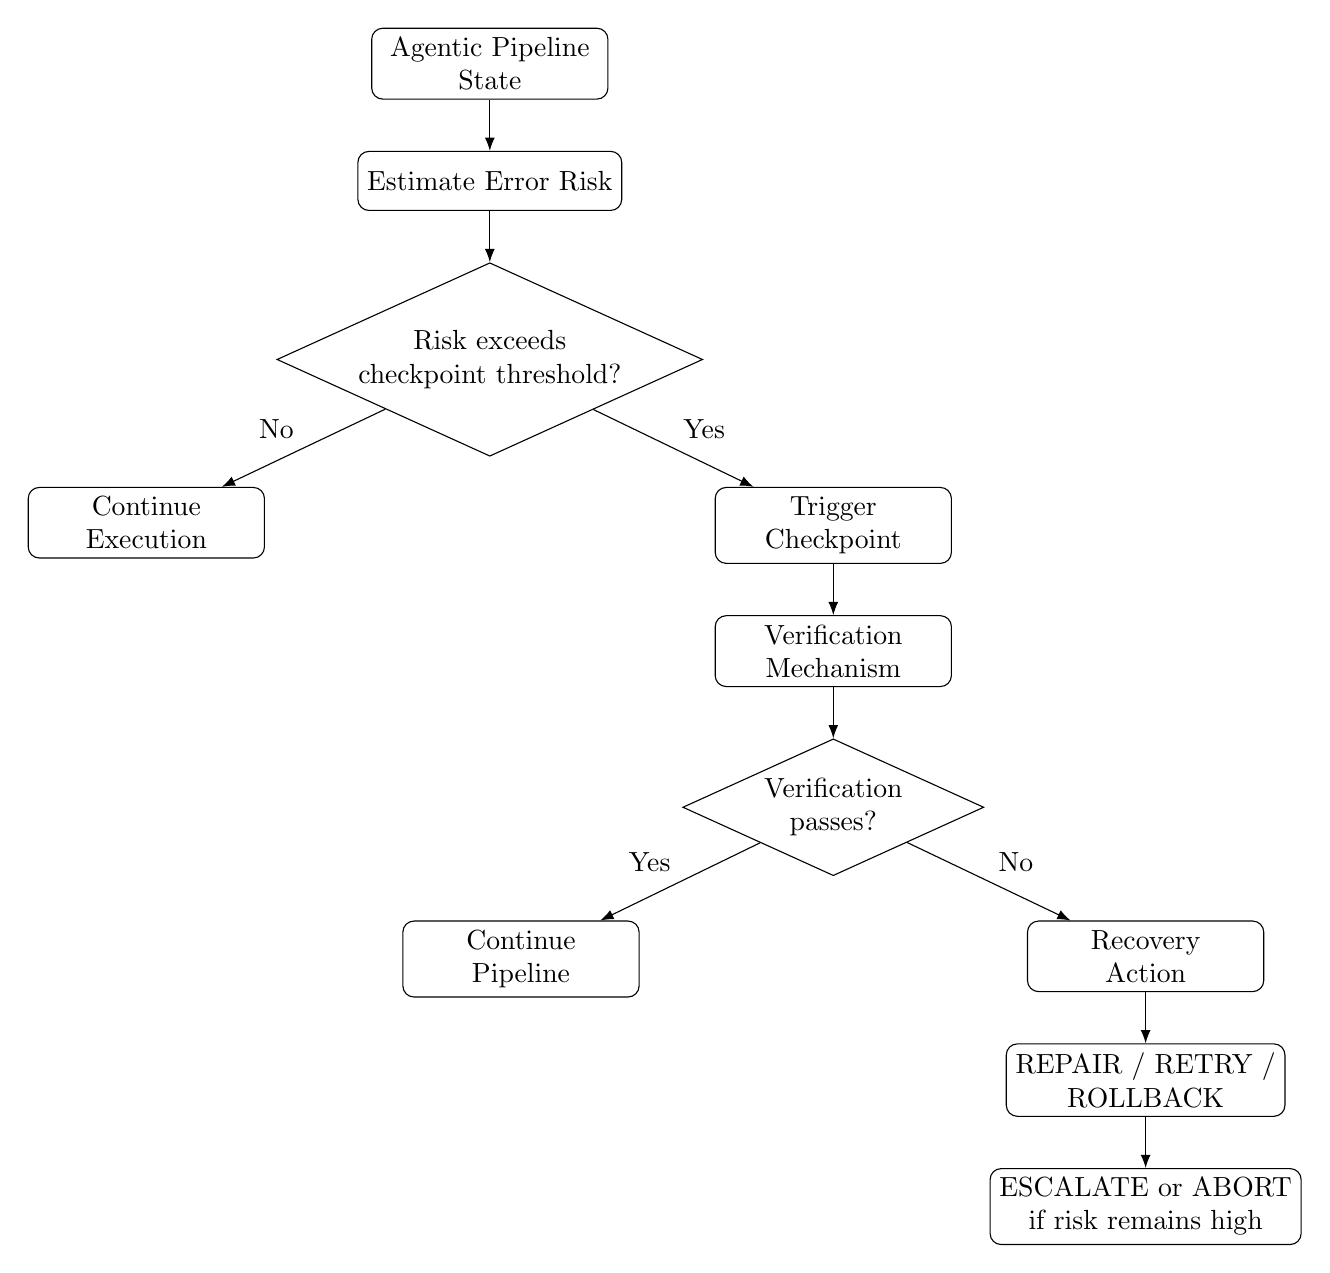
\begin{tikzpicture}[
    node distance=0.65cm,
    box/.style={
        draw,
        rounded corners,
        align=center,
        minimum width=3.0cm,
        minimum height=0.75cm
    },
    decision/.style={
        draw,
        diamond,
        aspect=2.2,
        align=center,
        inner sep=2pt
    },
    arrow/.style={->,>=Latex}
]

\node[box] (state) {Agentic Pipeline\\State};
\node[box, below=of state] (risk) {Estimate Error Risk};

\node[decision, below=of risk] (decision) {Risk exceeds\\checkpoint threshold?};

\node[box, below left=1.0cm and 1.5cm of decision] (continue)
{Continue\\Execution};

\node[box, below right=1.0cm and 1.5cm of decision] (checkpoint)
{Trigger\\Checkpoint};

\node[box, below=of checkpoint] (verify)
{Verification\\Mechanism};

\node[decision, below=of verify] (result) {Verification\\passes?};

\node[box, below left=1.0cm and 1.5cm of result] (pass)
{Continue\\Pipeline};

\node[box, below right=1.0cm and 1.5cm of result] (fail)
{Recovery\\Action};

\node[box, below=of fail] (recovery)
{REPAIR / RETRY /\\ROLLBACK};

\node[box, below=of recovery] (escalate)
{ESCALATE or ABORT\\if risk remains high};

\draw[arrow] (state) -- (risk);
\draw[arrow] (risk) -- (decision);

\draw[arrow] (decision) -- node[above left]{No} (continue);
\draw[arrow] (decision) -- node[above right]{Yes} (checkpoint);

\draw[arrow] (checkpoint) -- (verify);
\draw[arrow] (verify) -- (result);

\draw[arrow] (result) -- node[above left]{Yes} (pass);
\draw[arrow] (result) -- node[above right]{No} (fail);

\draw[arrow] (fail) -- (recovery);
\draw[arrow] (recovery) -- (escalate);

\end{tikzpicture}%
}
\caption{Risk-adaptive checkpoint decision and recovery flow.}
\label{fig:risk-adaptive-flow}
\end{figure}

The resulting risk-adaptive decision process is illustrated in
Figure~\ref{fig:risk-adaptive-flow}.

\subsection{Deterministic versus model-based verification}
\label{sec:deterministic-model-verification}

Where deterministic validation is possible, it can provide a strong basis for
verification. Examples include schema validation, range checks, type checking,
mathematical constraints, and consistency rules.

Model-based verification can be useful when deterministic rules are difficult
to define. However, the verifier itself may produce incorrect judgments. A
simple confidence-based condition can be expressed as

\begin{equation}
P(\text{correct})<\tau
\label{eq:confidence-threshold}
\end{equation}

where $\tau$ is a minimum confidence threshold.

\subsection{Independent verification}
\label{sec:independent-verification}

Independent verification reduces the possibility that the same reasoning
process produces both an error and its verification. Verification can be
performed by a separate model, deterministic program, retrieval system, or
human reviewer.

\section{Error Recovery and Checkpoint Actions}
\label{sec:error-recovery}

A checkpoint is useful only if detection can lead to an appropriate recovery
action. Depending on the type and severity of the detected error, the system
may repair the state, retry the operation, roll back to an earlier valid
state, escalate the decision to another component, or abort execution.

Rollback restores the last verified state, which can be represented as

\begin{equation}
S_i \rightarrow S_{i-k}
\label{eq:rollback}
\end{equation}

Rollback is valuable when an agent has performed reversible state-changing
operations. Escalation transfers the decision to a human or a
higher-assurance system when the estimated probability of correctness falls
below an acceptable threshold, or when the consequence of an error exceeds a
defined limit. This is especially important for high-impact actions where
autonomous recovery may itself introduce additional risk.

\section{Current Approaches and Developments}
\label{sec:current-approaches}

\subsection{Process supervision}
\label{sec:process-supervision-approach}

Process supervision evaluates intermediate reasoning steps instead of relying
only on the final answer. This approach is particularly relevant to checkpoint
design because intermediate errors can be detected before they propagate
\cite{lightman2023verify}.

\subsection{Self-consistency}
\label{sec:self-consistency}

Self-consistency samples multiple reasoning paths and selects an answer based
on agreement among those paths \cite{wang2023selfconsistency}. It can provide
an additional verification signal, although agreement between multiple outputs
does not guarantee correctness.

\subsection{Retrieval-grounded verification}
\label{sec:retrieval-verification}

Retrieval-grounded methods compare generated information against retrieved
evidence. RAGAs provides evaluation measures for retrieval augmented generation
systems \cite{es2024ragas}. External evidence can help reduce unsupported
claims and provide a basis for verification.

\subsection{LLM-as-a-judge}
\label{sec:llm-judge}

LLM-based judges can evaluate generated responses according to specified
criteria. Zheng et al. studied the use of LLMs as judges and evaluated their
agreement with human judgments \cite{zheng2023judge}. However, model-based
judges may share biases or failure modes with the systems they evaluate.

\subsection{Red-team-based verification}
\label{sec:red-team-verification}

Red-team approaches intentionally attempt to expose weaknesses in AI systems.
Perez et al. investigated the use of language models for red teaming language
models \cite{perez2022redteam}. Such techniques can complement checkpoint
mechanisms by testing whether verification controls can withstand adversarial
or unexpected inputs.

\section{Proposed Verification-Checkpoint Framework}
\label{sec:proposed-framework}

The proposed framework organizes verification around the major components of an
agentic execution: intent, planning, actions, observations, state, and
outcomes. Rather than treating verification as a single final-stage operation,
the framework introduces checkpoints at selected high-risk transitions.

A checkpoint may therefore be associated with the task definition, a generated
plan, a tool call, an observation, a state update, or the final result. Each
checkpoint evaluates a verification predicate and selects an appropriate action
based on the result.

The resulting VCP-AI architecture is illustrated in
Figure~\ref{fig:vcp-ai-architecture}.

\begin{figure}[htbp]
\centering
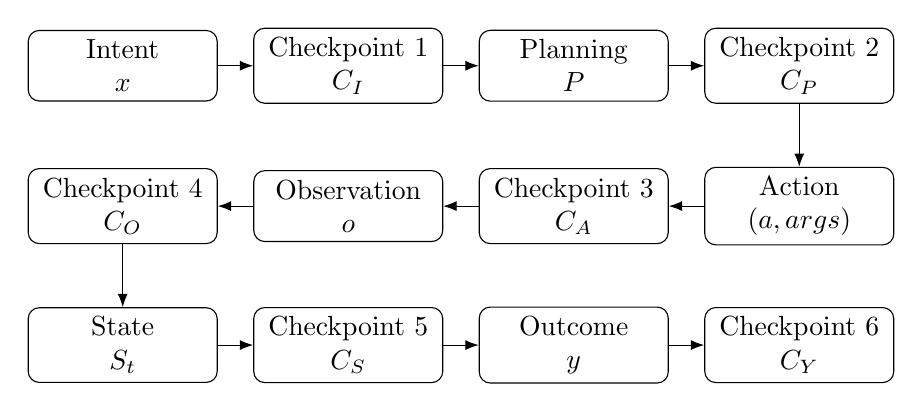
\begin{tikzpicture}[
    node distance=0.45cm,
    box/.style={
        draw,
        rounded corners,
        align=center,
        minimum width=2.4cm,
        minimum height=0.75cm
    },
    checkpoint/.style={
        draw,
        rounded corners,
        align=center,
        minimum width=2.4cm,
        minimum height=0.75cm
    },
    arrow/.style={->,>=Latex}
]

\node[box] (intent) {Intent\\$x$};
\node[checkpoint, right=of intent] (ci) {Checkpoint 1\\$C_I$};

\node[box, right=of ci] (plan) {Planning\\$P$};
\node[checkpoint, right=of plan] (cp) {Checkpoint 2\\$C_P$};

\node[box, below=0.8cm of cp] (action) {Action\\$(a,args)$};
\node[checkpoint, left=of action] (ca) {Checkpoint 3\\$C_A$};

\node[box, left=of ca] (observation) {Observation\\$o$};
\node[checkpoint, left=of observation] (co) {Checkpoint 4\\$C_O$};

\node[box, below=0.8cm of co] (state) {State\\$S_t$};
\node[checkpoint, right=of state] (cs) {Checkpoint 5\\$C_S$};

\node[box, right=of cs] (outcome) {Outcome\\$y$};
\node[checkpoint, right=of outcome] (cy) {Checkpoint 6\\$C_Y$};

\draw[arrow] (intent) -- (ci);
\draw[arrow] (ci) -- (plan);
\draw[arrow] (plan) -- (cp);
\draw[arrow] (cp) -- (action);
\draw[arrow] (action) -- (ca);
\draw[arrow] (ca) -- (observation);
\draw[arrow] (observation) -- (co);
\draw[arrow] (co) -- (state);
\draw[arrow] (state) -- (cs);
\draw[arrow] (cs) -- (outcome);
\draw[arrow] (outcome) -- (cy);

\end{tikzpicture}
\caption{VCP-AI layered verification architecture for agentic AI pipelines.}
\label{fig:vcp-ai-architecture}
\end{figure}

\subsection{Checkpoint effectiveness}
\label{sec:checkpoint-effectiveness}

The effectiveness of a verification mechanism can be evaluated using several
metrics.

Detection recall can be represented as

\begin{equation}
DR=\frac{TP}{TP+FN}
\label{eq:detection-recall}
\end{equation}

where $TP$ denotes true positives and $FN$ denotes false negatives.

False-positive rate can be represented as

\begin{equation}
FPR=\frac{FP}{FP+TN}
\label{eq:false-positive-rate}
\end{equation}

where $FP$ denotes false positives and $TN$ denotes true negatives.

Containment rate can be defined as

\begin{equation}
CR=
\frac{\text{errors prevented from reaching final action}}
{\text{errors introduced}}
\label{eq:containment-rate}
\end{equation}

Verification overhead can be represented as

\begin{equation}
VO=
\frac{\text{additional latency or computational cost}}
{\text{baseline cost}}
\label{eq:verification-overhead}
\end{equation}

Finally, the silent-error rate can be expressed as

\begin{equation}
SER=
\frac{\text{undetected harmful errors}}
{\text{total execution opportunities}}
\label{eq:silent-error-rate}
\end{equation}

These measures allow verification mechanisms to be evaluated not only according
to whether they detect errors, but also according to their cost and ability to
prevent errors from reaching consequential actions.

\section{Research Challenges and Limitations}
\label{sec:limitations}

\subsection{The verifier can fail}
\label{sec:verifier-failure}

A verification mechanism is itself a component of the system and can therefore
produce incorrect judgments. A verifier may fail to detect an error, incorrectly
reject a correct result, or misinterpret the state being evaluated.

\subsection{Correlated errors}
\label{sec:correlated-errors}

Independent verification is difficult when multiple verification components
share the same model, training data, assumptions, or information sources.
Correlated failures can therefore allow the same error to pass through multiple
checkpoints.

\subsection{Verification cost}
\label{sec:verification-cost}

Additional verification increases computational cost and latency. The total
execution cost can be represented as

\begin{equation}
T_{\mathrm{total}}
=
T_{\mathrm{agent}}
+
\sum_i T_{C_i}
\label{eq:total-cost}
\end{equation}

where $T_{\mathrm{agent}}$ is the original agent execution time and $T_{C_i}$
represents the time associated with checkpoint $i$. Excessive checkpointing
may reduce the efficiency and responsiveness of an agentic system. The
challenge is therefore to identify checkpoints that provide meaningful
reliability improvements without imposing unnecessary overhead.

\subsection{Non-deterministic environments}
\label{sec:nondeterministic-environments}

Agentic systems may operate in environments where actions produce different
results at different times. Verification must therefore account for uncertainty
and distinguish genuine errors from valid environmental variation.

\subsection{Difficulties in defining ground truth}
\label{sec:ground-truth}

Some agentic tasks do not have a single objectively correct intermediate state.
In such cases, verification requires task-specific criteria, external evidence,
or human judgment. Defining reliable ground truth is therefore an important
research challenge.

\section{Research Gaps and Future Directions}
\label{sec:future-work}

\subsection{Standardized silent-error benchmarks}
\label{sec:silent-error-benchmarks}

Existing agent benchmarks evaluate overall task performance, but systematic
benchmarks specifically designed to measure silent-error detection and
containment remain necessary. Such benchmarks should identify where errors are
introduced, whether they are detected, and whether they reach the final action.

\subsection{Causal error-trace datasets}
\label{sec:causal-error-datasets}

Datasets containing complete execution traces could support research into the
causal relationships between intermediate errors and final outcomes. Such
traces can be represented as

\begin{equation}
\tau=(S_0,A_1,O_1,\ldots,A_n,O_n,S_n)
\label{eq:trajectory}
\end{equation}

where $S_i$ represents a system state, $A_i$ represents an action, and $O_i$
represents an observation. Such datasets could annotate the first erroneous
state, error type, detection point, propagation path, final consequence, and
recovery outcome, enabling research into causal fault localization rather
than final-answer classification alone.

\subsection{Adaptive checkpoint scheduling}
\label{sec:adaptive-checkpoints}

Future systems could dynamically determine when checkpoints are required based
on estimated risk, task characteristics, state uncertainty, and downstream
impact. A checkpoint can be triggered when the estimated risk exceeds the
cost of verification:

\begin{equation}
\text{Checkpoint if }
P(E_i)\times I_i>\lambda C_i
\label{eq:checkpoint-rule}
\end{equation}

where $\lambda$ controls the trade-off between risk and verification cost.
The overall checkpoint-selection problem can then be formulated as

\begin{equation}
\operatorname{minimize}\quad
\operatorname{Cost}(C)
+
\lambda\times\operatorname{ResidualRisk}(C)
\label{eq:checkpoint-optimization}
\end{equation}

where $C$ denotes the selected set of checkpoints. This formalization could
allow verification resources to be concentrated at high-risk points, and
could lead to learned checkpoint schedulers.

\subsection{Fault-injection testing for agents}
\label{sec:fault-injection}

Fault injection can intentionally introduce errors into agentic execution in
order to evaluate whether checkpoint mechanisms detect and contain them. Such
testing could provide a systematic way to measure robustness.

\subsection{Verification under adversarial conditions}
\label{sec:adversarial-verification}

Verification mechanisms should also be evaluated against adversarial inputs and
attempts to bypass safety controls. Red-team approaches can provide one method
for identifying weaknesses in checkpoint systems.

\subsection{Human intervention as a calibrated resource}
\label{sec:human-intervention}

Human review should be treated as a limited resource rather than a universal
fallback. Future systems could escalate to a human only when

\begin{equation}
U(\text{autonomous action})
<
U(\text{human review})
\label{eq:human-review}
\end{equation}

where $U$ represents the expected utility of the respective action, taking
into account the probability of error, its consequence, latency, and review
cost. This would transform human oversight from a generic fallback into a
risk-calibrated verification mechanism.

\section{Conclusion}
\label{sec:conclusion}

Agentic AI systems introduce new reliability challenges because errors can occur
at intermediate stages and propagate without producing explicit failures. Silent
errors are particularly problematic because they may remain undetected until
they influence a consequential final action.

Verification checkpoints provide a mechanism for detecting and containing such
errors during execution rather than relying exclusively on final-output
evaluation. The framework proposed in this paper organizes verification around
intent, planning, actions, observations, state, and outcomes. It also emphasizes
risk-adaptive checkpoint placement, independent verification, and explicit
recovery actions.

The risk-adaptive placement discussed in
Section~\ref{sec:risk-adaptive} complements the layered architecture described
in Section~\ref{sec:five-layer}. The verification predicates described in
Equation~\ref{eq:verification-predicate} and the checkpoint action model in
Equation~\ref{eq:checkpoint-actions} provide formal representations of these
controls.

The effectiveness of checkpoint mechanisms depends not only on their ability to
detect errors but also on their cost, independence, robustness, and ability to
trigger appropriate recovery actions. Important challenges include verifier
failure, correlated errors, verification overhead, non-deterministic
environments, and the absence of clearly defined ground truth.

Future research should therefore focus on standardized silent-error benchmarks,
causal error-trace datasets, adaptive checkpoint scheduling, fault-injection
testing, adversarial verification, and calibrated human intervention. These
directions can help establish verification checkpoints as a systematic
reliability mechanism for increasingly autonomous AI systems.

\clearpage

\bibliographystyle{unsrt}

\nocite{yao2023react}
\nocite{schick2023toolformer}
\nocite{wu2023autogen}
\nocite{liu2024agentbench}
\nocite{jimenez2024swebench}
\nocite{mohammadi2025evaluation}
\nocite{yehudai2026survey}
\nocite{wei2022cot}
\nocite{wang2023selfconsistency}
\nocite{lightman2023verify}
\nocite{manakul2023selfcheckgpt}
\nocite{min2023factscore}
\nocite{es2024ragas}
\nocite{zheng2023judge}
\nocite{liu2024lost}
\nocite{perez2022redteam}
\nocite{kim2026agentic}

\bibliography{references}

\end{document}